%%=================================================%%
%%						TITRE DU DOCUMENT (1 PAGE)
%							  Pas totalement fini
%%=================================================%%

\begin{titlepage}
\begin{center}

% Upper part of the page. The '~' is needed because only works if a paragraph has started.


\includegraphics[width=0.60\textwidth]{./page_de_garde/logo_ups.png}~\\[1cm]

\textsc{\LARGE Université Paul Sabatier}\\[1.5cm]

\textsc{\Large \bf Modèle Temporel avancé }\\[0.5cm]

% Title
\HRule \\[0.4cm]

{\huge \bfseries  - TP : \textsc{Système de Traitement Automatisé} -}

\HRule \\[1.5cm]

% Author and supervisor
\begin{minipage}{0.4\textwidth}
\begin{flushleft} \large
\emph{Auteurs:}\\
Lucien \textsc{Rakotomalala}\\
David \textsc{Tocaven}\\
\end{flushleft}
\end{minipage}
\begin{minipage}{0.58\textwidth}
\begin{flushright} \large
\emph{Encadrant:} \\
\textbf{ Pauline \textsc{Ribot}}\\
\textbf{ Euriell \textsc{Le Corronc}}
\textbf{ Michel \textsc{Combacau}}
\end{flushright}
\end{minipage}
\newline
\newline
\vfill
% une éventuelle image
\fbox{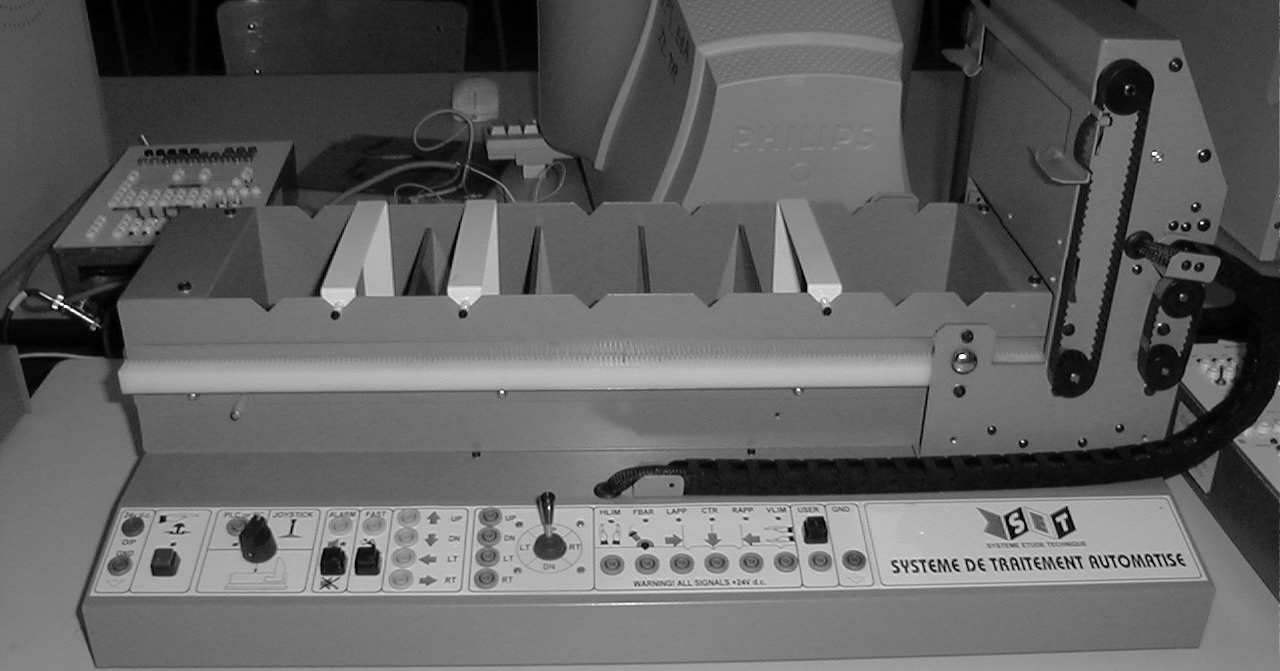
\includegraphics[width=.6\textwidth]{./page_de_garde/M2ASTR-TP-MACSED-STA.jpg}}~\\[1cm]

\vfill
% logo fsi & eea
\begin{tabular}{cc}
   
\includegraphics[height=2cm]{./page_de_garde/logo_fsi.png} \hspace{2cm} &
    \hspace{2cm}
   
\includegraphics[height=2cm]{./page_de_garde/logo_eea.jpg} \\
\end{tabular}

% Bottom of the page
{\large \today}

\end{center}
\end{titlepage}
